\documentclass[french]{report}
\usepackage[T1]{fontenc}
\usepackage[utf8]{inputenc}
\usepackage{lmodern}
\usepackage[a4paper]{geometry}
\usepackage{babel}
\usepackage{graphicx}
\usepackage{hyperref}

\renewcommand{\thesection}{\arabic{section}}

% Title Page
\title{INFOM218 - DBRE - Groupe 2 \\ \Huge Étape 1}
\author{BENIMEDOURENE, Charles \and CAUCHETEUR, Maxime \and DECROP, Alix \and DIERICKX, Jeremie \and JACOBS, Pierre}
\date{{\large Université de Namur} \\ \today}

\hypersetup{linktoc=all}

\begin{document}
	
	\maketitle
	\newpage
	\tableofcontents
	
	\newpage
	
	\section{Smoke}
	
	\textit{Smoke} est une application Android de communication chiffrée entre participants. Celle-ci n'est cependant pas vouée à être utilisée en situation réelle, mais est plus une \textit{expérimentation pour les curieux}. Celle-ci est écrite en Java et est disponible à cette adresse: \url{https://github.com/textbrowser/smoke}. Elle dispose d'une base de données \textit{SQLite}. Celle-ci est par ailleurs composée de douze tables différentes.
	
	L'objectif de ce document est de reconstruire les schémas physique, logique et conceptuel de la base de données à l'aide de l'outil \textit{SQLInspect} et de les exprimer grâce au langage de modélisation \textit{HyDRa}. Il propose également une simulation de découverte de clefs étrangères, afin de mesurer la facilité à retrouver lesdites clefs si elles n'étaient pas définies directement dans les requêtes \textit{"CREATE TABLE"}.

	\section{Schémas}
	\section{Découverte des clefs étrangères}
	
	Cette section se concentre sur la découverte des clefs étrangères présentes dans la base de données. La majorité de celles-ci sont explicitement décrites dans les requêtes \textit{"CREATE TABLE"}. 
	
	\begin{figure}[h!]
		\centering
		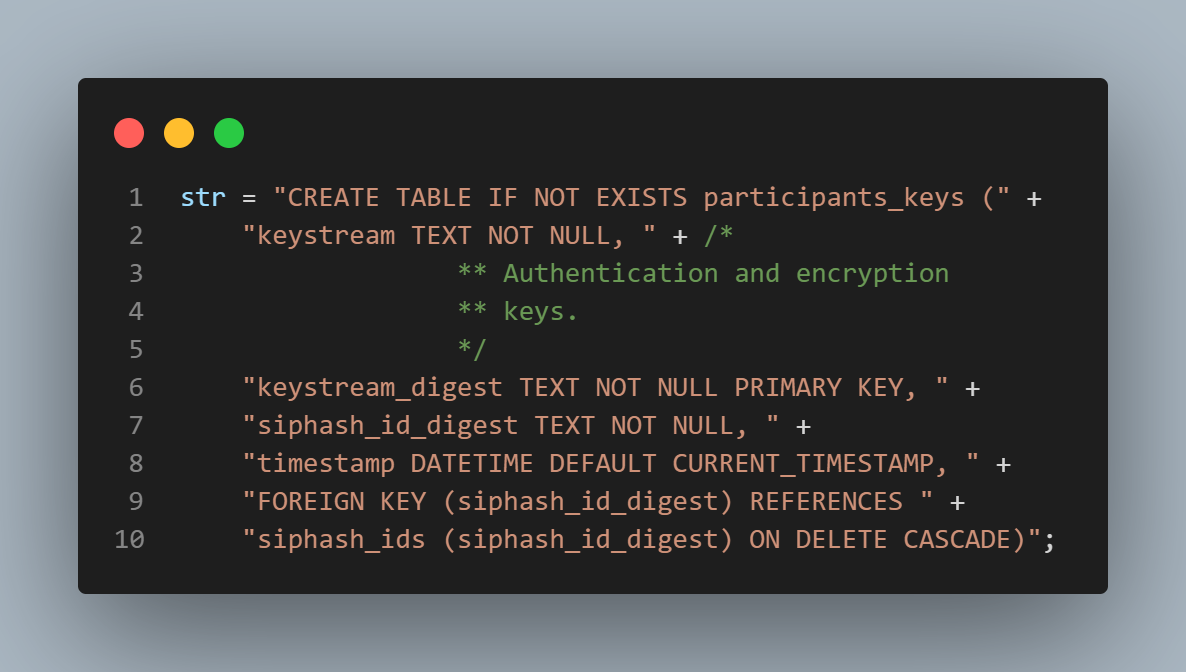
\includegraphics[width=0.75\textwidth]{imgs/create_table.png}
		\caption{Exemple de requête \textit{CREATE TABLE}}
		\label{fig::create_table}
	\end{figure}

	La figure \ref{fig::create_table} montre bien que certaines des clefs étrangères sont explicitement définies à la création des tables: \textit{FOREIGN KEY (siphash\_id\_digest) REFERENCES siphash\_ids (siphash\_id\_digest)}. Dans cet exemple, la table \textit{participants\_keys} possède une référence à la table \textit{siphash\_ids} grâce à son champ \textit{siphash\_id\_digest}. 
	
	\subsection{Clefs explicitement définies}
	
	Ci-dessous la liste des clefs étrangères explicitement définies, représentées sous la forme \newline <table>.<clef\_etrangere> $\rightarrow$ <table>.<champ> :
	
	\begin{itemize}
		\item arson\_keys.siphash\_id\_digest $\rightarrow$ siphash\_ids.siphash\_id\_digest;
		\item participants.siphash\_id\_digest $\rightarrow$ siphash\_ids.siphash\_id\_digest;
		\item participants\_keys.siphash\_id\_digest $\rightarrow$ siphash\_ids.siphash\_id\_digest;
		\item participants\_messages.siphash\_id\_digest $\rightarrow$ siphash\_ids.siphash\_id\_digest.
	\end{itemize}

	On notera tout de même que l'ensemble de ces clefs étrangères référencent le champ \textit{siphash\_id\_digest} de la table \textit{siphash\_ids}. Dans la suite de cette section, nous ferons l'hypothèse que ces clefs étrangères ne sont pas explicitement définies.
	
	\subsection{Simulation de découverte}
	
	En explorant le schéma généré par \textit{SQLInspect}, l'on se rend compte que de quelques champs dispersés dans différentes tables portent des noms évocateurs et sont de bons candidats pour être des clefs étrangères. 
	
	\paragraph{siphash\_id\_digest}{Les tables \textit{arson\_keys}, \textit{participants}, \textit{participants\_keys}, \newline \textit{participants\_messages} et \textit{siphash\_ids}} possèdent toutes un champ nommé \textit{siphash\_id\_digest}. Étant donné qu'une de ces tables se nomme \textit{siphash\_ids}, il est raisonnable de faire l'hypothèse que la table qui contient la référence \textit{siphash\_id\_digest} est effectivement la table \textit{siphash\_ids}. Par conséquent, les autres tables susmentionnées possèderaient effectivement la référence de ce champ-là comme clef étrangère.
	\paragraph{neighbor\_oid}{La table \textit{outbound\_queue} possède un champ nommé \textit{neighbor\_oid}, qui coïncide singulièrement avec le champ \textit{oid} de la table \textit{neighbor}. Bien que la convention de nommage soit différente par rapport aux clefs étrangères \textit{siphash\_id\_digest}, il apparait comme évident que le champ \textit{neighbor\_oid} est effectivement un clef étrangère du champ \textit{oid} de la table \textit{neighbor}. En analysant la méthode \textit{enqueueOutboundMessage} du fichier \textit{Database.java}, il apparait bel et bien que l'\textit{oid} est ajouté après avoir récupéré les différents \textit{oid} de la table \textit{neighbor}, confirmant à nouveau que \textit{neighbor\_oid} est bel et bien une clef étrangère.}
	\paragraph{siphash\_id}{Le champ \textit{siphash\_id} de la table \textit{participants} est également similaire au champ \textit{siphash\_id} de la table \textit{siphash\_ids}. Il est possible que ce champ soit également une clef étrangère. Cependant, en investigant le code source, il apparait que le champ \textit{siphash\_id} de la table \textit{participants} est uniquement utilisé dans la mise à jour des boites de dialogue des conversations entre participants. Par conséquent, le champ susmentionné ne semble pas être une clef étrangère.}
	
	
	\paragraph{}{Il est possible que d'autres clefs étrangères se cachent dans le code source. Cependant, aucun autre nom de champ n'apparait de manière flagrante comme candidat pour être une clef étrangère. De plus, le code source étant non commenté et de manière plus générale complexe à comprendre, il a été décidé d'arrêter la recherche de clefs étrangères à celles trouvées précédemment.}
	
	
\end{document}